\documentclass[10pt,a4paper]{article}\usepackage[]{graphicx}\usepackage[]{color}
%% maxwidth is the original width if it is less than linewidth
%% otherwise use linewidth (to make sure the graphics do not exceed the margin)
\makeatletter
\def\maxwidth{ %
  \ifdim\Gin@nat@width>\linewidth
    \linewidth
  \else
    \Gin@nat@width
  \fi
}
\makeatother

\definecolor{fgcolor}{rgb}{0.345, 0.345, 0.345}
\newcommand{\hlnum}[1]{\textcolor[rgb]{0.686,0.059,0.569}{#1}}%
\newcommand{\hlstr}[1]{\textcolor[rgb]{0.192,0.494,0.8}{#1}}%
\newcommand{\hlcom}[1]{\textcolor[rgb]{0.678,0.584,0.686}{\textit{#1}}}%
\newcommand{\hlopt}[1]{\textcolor[rgb]{0,0,0}{#1}}%
\newcommand{\hlstd}[1]{\textcolor[rgb]{0.345,0.345,0.345}{#1}}%
\newcommand{\hlkwa}[1]{\textcolor[rgb]{0.161,0.373,0.58}{\textbf{#1}}}%
\newcommand{\hlkwb}[1]{\textcolor[rgb]{0.69,0.353,0.396}{#1}}%
\newcommand{\hlkwc}[1]{\textcolor[rgb]{0.333,0.667,0.333}{#1}}%
\newcommand{\hlkwd}[1]{\textcolor[rgb]{0.737,0.353,0.396}{\textbf{#1}}}%

\usepackage{framed}
\makeatletter
\newenvironment{kframe}{%
 \def\at@end@of@kframe{}%
 \ifinner\ifhmode%
  \def\at@end@of@kframe{\end{minipage}}%
  \begin{minipage}{\columnwidth}%
 \fi\fi%
 \def\FrameCommand##1{\hskip\@totalleftmargin \hskip-\fboxsep
 \colorbox{shadecolor}{##1}\hskip-\fboxsep
     % There is no \\@totalrightmargin, so:
     \hskip-\linewidth \hskip-\@totalleftmargin \hskip\columnwidth}%
 \MakeFramed {\advance\hsize-\width
   \@totalleftmargin\z@ \linewidth\hsize
   \@setminipage}}%
 {\par\unskip\endMakeFramed%
 \at@end@of@kframe}
\makeatother

\definecolor{shadecolor}{rgb}{.97, .97, .97}
\definecolor{messagecolor}{rgb}{0, 0, 0}
\definecolor{warningcolor}{rgb}{1, 0, 1}
\definecolor{errorcolor}{rgb}{1, 0, 0}
\newenvironment{knitrout}{}{} % an empty environment to be redefined in TeX

\usepackage{alltt}
\usepackage[latin1]{inputenc}
\usepackage{amsmath}
\usepackage{amsfonts}
\usepackage{amssymb}
\author{Erika Martínez}
\title{Guías prácticas}
\IfFileExists{upquote.sty}{\usepackage{upquote}}{}
\begin{document}

\maketitle
\newpage

UNIDAD 3: Pr?ctica 14 - Distribuciones de probabilidad discreta 

CALCULO DE PROBABILIDADES.

Ejemplo 1:
\begin{knitrout}
\definecolor{shadecolor}{rgb}{0.969, 0.969, 0.969}\color{fgcolor}\begin{kframe}
\begin{alltt}
\hlcom{#Si un estudiante responde al azar a un examen de 8 preguntas de verdadero o falso. }
\hlcom{#a) ?Cu?l es la probabilidad de que acierte 4?}
\hlkwd{dbinom}\hlstd{(}\hlnum{4}\hlstd{,}\hlnum{8}\hlstd{,}\hlnum{0.5}\hlstd{)}
\end{alltt}
\begin{verbatim}
## [1] 0.2734375
\end{verbatim}
\begin{alltt}
\hlcom{#b) ?Cu?l es la probabilidad de que acierte a lo sumo 2?}
\hlstd{x} \hlkwb{<-} \hlnum{2}\hlstd{; n}\hlkwb{=}\hlnum{8}\hlstd{; p}\hlkwb{=}\hlnum{1}\hlopt{/}\hlnum{2}
\hlkwd{pbinom}\hlstd{(x,} \hlkwc{size} \hlstd{= n,} \hlkwc{prob} \hlstd{= p,} \hlkwc{lower.tail}\hlstd{=}\hlnum{TRUE}\hlstd{)}
\end{alltt}
\begin{verbatim}
## [1] 0.1445313
\end{verbatim}
\begin{alltt}
\hlcom{#c) ?Cu?l es la probabilidad de que acierte 5 o m?s?}
\hlstd{x} \hlkwb{<-} \hlnum{4}\hlstd{; n}\hlkwb{=}\hlnum{8}\hlstd{; p}\hlkwb{=}\hlnum{1}\hlopt{/}\hlnum{2}

\hlcom{#primera forma }
\hlstd{F} \hlkwb{<-} \hlnum{1} \hlopt{-} \hlkwd{pbinom}\hlstd{(x, n, p,} \hlkwc{lower.tail}\hlstd{=}\hlnum{TRUE}\hlstd{); F}
\end{alltt}
\begin{verbatim}
## [1] 0.3632813
\end{verbatim}
\begin{alltt}
\hlcom{#segunda forma }
\hlkwd{pbinom}\hlstd{(}\hlnum{4}\hlstd{,} \hlkwc{size}\hlstd{=}\hlnum{8}\hlstd{,} \hlkwc{prob}\hlstd{=}\hlnum{0.5}\hlstd{,} \hlkwc{lower.tail}\hlstd{=}\hlnum{FALSE}\hlstd{)}
\end{alltt}
\begin{verbatim}
## [1] 0.3632813
\end{verbatim}
\end{kframe}
\end{knitrout}

Ejemplo 2:
\begin{knitrout}
\definecolor{shadecolor}{rgb}{0.969, 0.969, 0.969}\color{fgcolor}\begin{kframe}
\begin{alltt}
\hlcom{#Una cierta ?rea de Estados Unidos es afectada, en promedio, por 6 huracanes al a?o. }
\hlcom{#Encuentre la probabilidad de que en un determinado a?o esta ?rea sea afectada por: }

\hlcom{#a) Menos de 4 huracanes.}
\hlstd{x} \hlkwb{<-} \hlnum{3}\hlstd{; mu} \hlkwb{<-} \hlnum{6}
\hlkwd{ppois}\hlstd{(x,} \hlkwc{lambda} \hlstd{= mu,} \hlkwc{lower.tail}\hlstd{=}\hlnum{TRUE}\hlstd{)}
\end{alltt}
\begin{verbatim}
## [1] 0.1512039
\end{verbatim}
\begin{alltt}
\hlcom{#b) Entre 6 y 8 huracanes}
\hlcom{#primera forma }
\hlkwd{sum}\hlstd{(}\hlkwd{dpois}\hlstd{(}\hlkwd{c}\hlstd{(}\hlnum{6}\hlstd{,}\hlnum{7}\hlstd{,}\hlnum{8}\hlstd{),}\hlkwc{lambda} \hlstd{=} \hlnum{6}\hlstd{))}
\end{alltt}
\begin{verbatim}
## [1] 0.4015579
\end{verbatim}
\begin{alltt}
\hlcom{# segunda forma restar las probabilidades acumuladas}
\hlstd{F8} \hlkwb{<-} \hlkwd{ppois}\hlstd{(}\hlnum{8}\hlstd{,} \hlkwc{lambda} \hlstd{=} \hlnum{6}\hlstd{,} \hlkwc{lower.tail}\hlstd{=}\hlnum{TRUE}\hlstd{)}
\hlstd{F5} \hlkwb{<-} \hlkwd{ppois}\hlstd{(}\hlnum{5}\hlstd{,}\hlkwc{lambda} \hlstd{=} \hlnum{6}\hlstd{,} \hlkwc{lower.tail}\hlstd{=}\hlnum{TRUE}\hlstd{)}
\hlstd{F8} \hlopt{-} \hlstd{F5}
\end{alltt}
\begin{verbatim}
## [1] 0.4015579
\end{verbatim}
\begin{alltt}
\hlcom{#c) Represente gr?ficamente la funci?n de probabilidad }
\hlcom{#de la variable aleatoria X que mide el n?mero de huracanes por a?o.}
\hlcom{#n <- 30 }
\hlcom{#genera 30 valores de una distribuci?n de Poisson con ??=6}
\hlstd{x} \hlkwb{<-} \hlkwd{rpois}\hlstd{(n,} \hlkwc{lambda}\hlstd{=mu)}

\hlcom{#calcula las probabilidades para cada valor generado }
\hlstd{y} \hlkwb{<-} \hlkwd{dpois}\hlstd{(x,} \hlkwc{lambda}\hlstd{=mu)}

\hlcom{#genera el gr?fico de distribuci?n }
\hlkwd{plot}\hlstd{(x, y,} \hlkwc{xlab}\hlstd{=}\hlstr{"x"}\hlstd{,} \hlkwc{ylab}\hlstd{=}\hlstr{"Funci?n de probalidad"}\hlstd{,}
\hlkwc{main}\hlstd{=}\hlstr{"Distribuci?n de Poisson: lambda = 6"}\hlstd{,}\hlkwc{type}\hlstd{=}\hlstr{"h"}\hlstd{)}

\hlcom{#une los puntos a las l?neas }
\hlkwd{points}\hlstd{(x, y,} \hlkwc{pch}\hlstd{=}\hlnum{21}\hlstd{)}
\end{alltt}
\end{kframe}
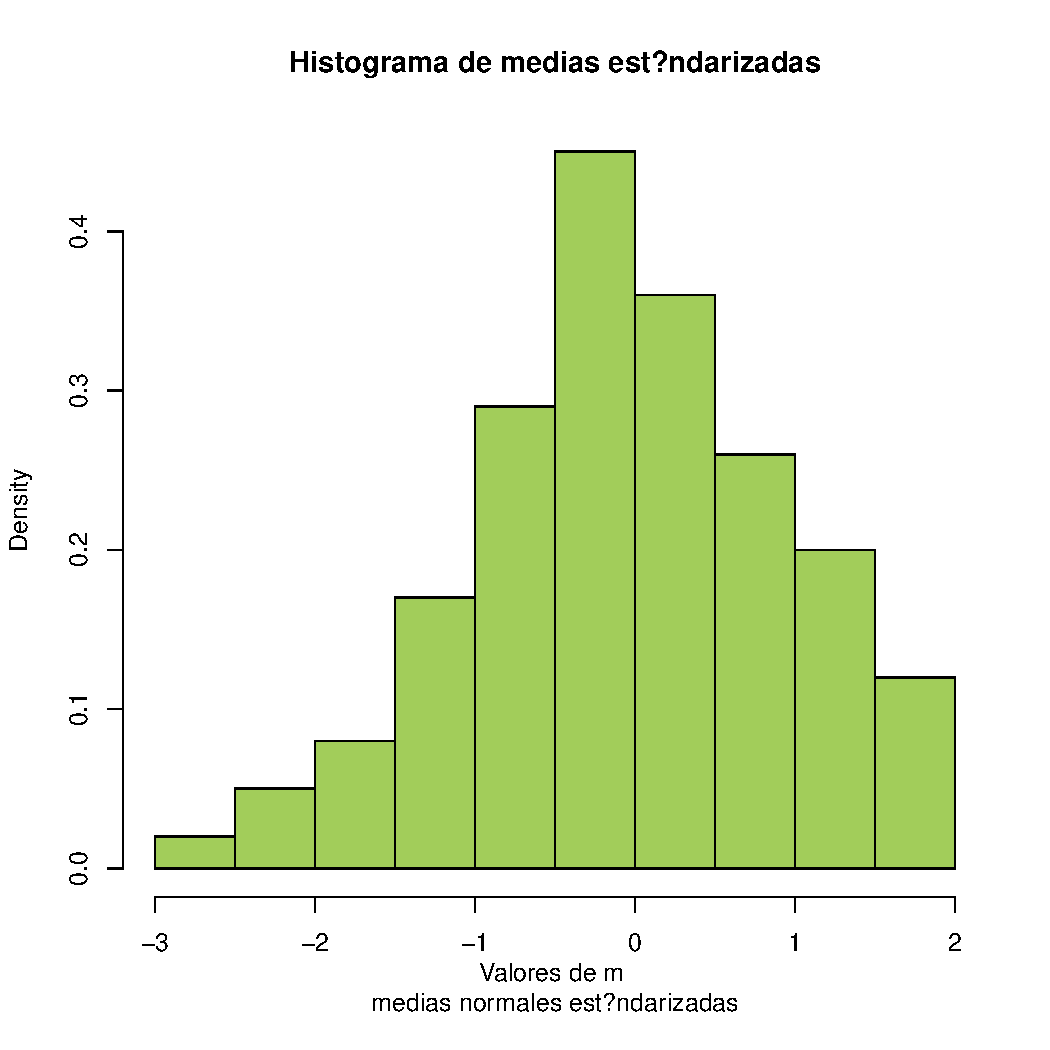
\includegraphics[width=\maxwidth]{figure/unnamed-chunk-2-1} 

\end{knitrout}

Ejemplo 3: 
\begin{knitrout}
\definecolor{shadecolor}{rgb}{0.969, 0.969, 0.969}\color{fgcolor}\begin{kframe}
\begin{alltt}
\hlcom{#En un juego se disponen 15 globos llenos de agua, delos que 4 tienen premio. Los participantes en el }
\hlcom{#juego, con los ojos vendados, golpean los globos con un bate por orden hasta que cada uno consigue romper2.}

\hlcom{#a) ?Cu?l es la probabilidad de que elprimer participante consiga un premio?}
\hlcom{# x define el n?mero de globos con premio}
\hlstd{x} \hlkwb{<-} \hlnum{0}\hlopt{:}\hlnum{2}\hlstd{; m} \hlkwb{=} \hlnum{11}\hlstd{; n} \hlkwb{<-} \hlnum{4}\hlstd{; k}\hlkwb{=}\hlnum{2}

\hlcom{# se construye la distribuci?n de frecuencias del n?mero de premios }
\hlstd{Tabla} \hlkwb{<-} \hlkwd{data.frame}\hlstd{(}\hlkwc{Probabilidad}\hlstd{=}\hlkwd{dhyper}\hlstd{(x, m, n, k))}
\hlkwd{rownames}\hlstd{(Tabla)} \hlkwb{<-} \hlkwd{c}\hlstd{(}\hlstr{"Ning?n premio"}\hlstd{,}\hlstr{"Solamente uno"}\hlstd{,} \hlstr{"Dos premios"}\hlstd{)}
\hlstd{Tabla}
\end{alltt}
\begin{verbatim}
##               Probabilidad
## Ning?n premio   0.05714286
## Solamente uno   0.41904762
## Dos premios     0.52380952
\end{verbatim}
\begin{alltt}
\hlcom{#b) Si el primer participante ha conseguido s?lo un premio, ?cu?l es la probabilidad de que el }
\hlcom{#segundo participante consiga otro?}
\hlstd{x} \hlkwb{=} \hlnum{1}\hlstd{; m}\hlkwb{=} \hlnum{10}\hlstd{; n}\hlkwb{=} \hlnum{3}\hlstd{; k}\hlkwb{=} \hlnum{2}\hlstd{;}
\hlkwd{dhyper}\hlstd{(x, m, n, k)}
\end{alltt}
\begin{verbatim}
## [1] 0.3846154
\end{verbatim}
\end{kframe}
\end{knitrout}

Ejemplo 4: 
\begin{knitrout}
\definecolor{shadecolor}{rgb}{0.969, 0.969, 0.969}\color{fgcolor}\begin{kframe}
\begin{alltt}
\hlcom{#Un vendedor de alarmas de hogar tiene ?xito enuna casa de cada diez que visita. }
\hlcom{#Calcula:}

\hlcom{#a) La probabilidad de que en un d?a determinado consiga vender la primera alarma en la sexta }
\hlcom{#casa que visita.}
\hlcom{# x define el n?mero de intentos fallidos }
\hlstd{x} \hlkwb{<-} \hlnum{0}\hlopt{:}\hlnum{5}\hlstd{; p}\hlkwb{=}\hlnum{0.1}

\hlcom{# creando la tabla de distribuci?n de frecuencias del n?mero de intentos fallidos antes de }
\hlcom{#obtener la primera venta. }
\hlstd{Tabla} \hlkwb{<-} \hlkwd{data.frame}\hlstd{(}\hlkwc{Probabilidad}\hlstd{=}\hlkwd{dgeom}\hlstd{(x,} \hlkwc{prob}\hlstd{=p))}

\hlcom{# nombrando las filas de la distribuci?n de frecuencias }
\hlkwd{rownames}\hlstd{(Tabla)} \hlkwb{<-} \hlkwd{c}\hlstd{(}\hlstr{"Venta en el primer intento"}\hlstd{,} \hlstr{"Venta en el segundo intento"}\hlstd{,}
\hlstr{"Venta en el tercer intento"}\hlstd{,} \hlstr{"Venta en el cuarto intento"}\hlstd{,}
\hlstr{"Venta en el quinto intento"}\hlstd{,} \hlstr{"Venta en el sexto intento"}\hlstd{)}
\hlstd{Tabla}
\end{alltt}
\begin{verbatim}
##                             Probabilidad
## Venta en el primer intento      0.100000
## Venta en el segundo intento     0.090000
## Venta en el tercer intento      0.081000
## Venta en el cuarto intento      0.072900
## Venta en el quinto intento      0.065610
## Venta en el sexto intento       0.059049
\end{verbatim}
\begin{alltt}
\hlcom{#b) La probabilidad de que no venda ninguna despu?s de siete viviendas visitadas.}
\hlstd{x}\hlkwb{=}\hlnum{0}\hlstd{; n}\hlkwb{=}\hlnum{7}\hlstd{; p}\hlkwb{=}\hlnum{0.1}
\hlkwd{dbinom}\hlstd{(x, n, p,} \hlkwc{log} \hlstd{=} \hlnum{FALSE}\hlstd{)}
\end{alltt}
\begin{verbatim}
## [1] 0.4782969
\end{verbatim}
\begin{alltt}
\hlcom{#c) Si se plantea vender tres alarmas, ?cu?l es la probabilidad deque consiga su objetivo en la }
\hlcom{#octava vivienda que visita?}
\hlstd{y} \hlkwb{<-} \hlnum{0}\hlopt{:}\hlnum{5}\hlstd{; r}\hlkwb{=}\hlnum{3}\hlstd{; p} \hlkwb{<-} \hlnum{0.1}
\hlstd{Tabla} \hlkwb{<-} \hlkwd{data.frame}\hlstd{(}\hlkwc{Probabilidad}\hlstd{=}\hlkwd{dnbinom}\hlstd{(y,} \hlkwc{size}\hlstd{=r,} \hlkwc{prob}\hlstd{=p))}
\hlkwd{rownames}\hlstd{(Tabla)} \hlkwb{<-} \hlnum{0}\hlopt{:}\hlnum{5}
\hlstd{Tabla}
\end{alltt}
\begin{verbatim}
##   Probabilidad
## 0   0.00100000
## 1   0.00270000
## 2   0.00486000
## 3   0.00729000
## 4   0.00984150
## 5   0.01240029
\end{verbatim}
\end{kframe}
\end{knitrout}

GENERACION DE MUESTRAS ALEATORIAS DE LAS DISTRIBUCIONES 
Ejemplo 1: 
\begin{knitrout}
\definecolor{shadecolor}{rgb}{0.969, 0.969, 0.969}\color{fgcolor}\begin{kframe}
\begin{alltt}
\hlcom{#Generar 100 n?meros aleatorios de una distribuci?n Binomial de par?metros n= 15 ensayos o pruebas }
\hlcom{#y una probabilidad de ?xito de 0.25. }
\hlcom{# Definir los par?metros apropiados }
\hlstd{n} \hlkwb{<-} \hlnum{15}\hlstd{; p} \hlkwb{<-} \hlnum{0.25}

\hlcom{# generar 100 n?meros aleatorios binomiales }
\hlstd{x} \hlkwb{=} \hlkwd{rbinom}\hlstd{(}\hlnum{100}\hlstd{, n, p); x}
\end{alltt}
\begin{verbatim}
##   [1] 4 2 6 3 5 5 2 3 7 5 3 3 3 2 6 5 3 4 3 4 4 5 3 4 6 2 8 4 3 2 2 4 2 4 3
##  [36] 3 5 3 4 8 2 4 2 6 7 3 9 5 2 6 6 5 4 3 2 3 2 1 5 1 5 5 6 2 2 4 3 3 2 3
##  [71] 4 5 4 2 4 2 4 1 5 4 5 3 4 2 4 2 7 1 6 4 4 4 4 5 2 1 1 3 3 5
\end{verbatim}
\begin{alltt}
\hlcom{# Histograma para la muestra aleatoria de tama?o 100 }
\hlkwd{hist}\hlstd{(x,} \hlkwc{main}\hlstd{=}\hlstr{"X ~ Binomial(n=15, p=0.25)"}\hlstd{,} \hlkwc{xlab}\hlstd{=}\hlstr{"X = N?mero de ?xitos"}\hlstd{,}
\hlkwc{ylab}\hlstd{=}\hlstr{"masa de probabilidad"}\hlstd{,} \hlkwc{probability}\hlstd{=}\hlnum{TRUE}\hlstd{,} \hlkwc{col}\hlstd{=}\hlstr{"black"}\hlstd{)}

\hlcom{# Graficar la funci?n de probabilidad te?rica, use la funci?n points(), }
\hlcom{#no debe cerrar el gr?fico obtenido con la instrucci?n anterior }
\hlstd{xvals}\hlkwb{=}\hlnum{0}\hlopt{:}\hlstd{n;} \hlkwd{points}\hlstd{(xvals,} \hlkwd{dbinom}\hlstd{(xvals, n, p),} \hlkwc{type}\hlstd{=}\hlstr{"h"}\hlstd{,} \hlkwc{lwd}\hlstd{=}\hlnum{3}\hlstd{)}
\hlkwd{points}\hlstd{(xvals,} \hlkwd{dbinom}\hlstd{(xvals, n, p),} \hlkwc{type}\hlstd{=}\hlstr{"p"}\hlstd{,} \hlkwc{lwd}\hlstd{=}\hlnum{3}\hlstd{)}
\end{alltt}
\end{kframe}
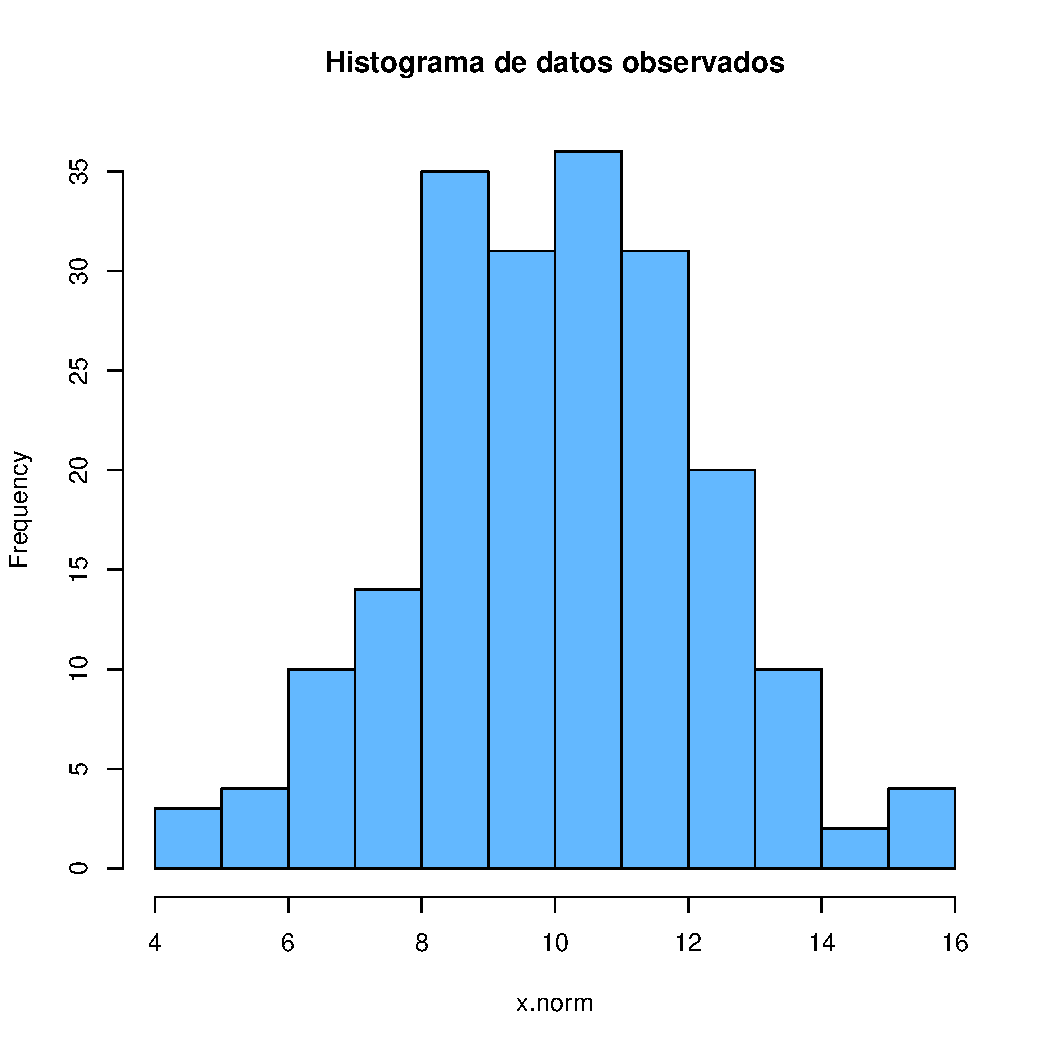
\includegraphics[width=\maxwidth]{figure/unnamed-chunk-5-1} 

\end{knitrout}

Ejemplo 2: 
\begin{knitrout}
\definecolor{shadecolor}{rgb}{0.969, 0.969, 0.969}\color{fgcolor}\begin{kframe}
\begin{alltt}
\hlcom{#Generar 100 n?meros aleatorios de una distribuci?n Poisson con 200000 }
\hlcom{#ensayos o pruebas y una probabilidad de ?xito de 3/100000 }

\hlcom{# Definir los par?metros apropiados }
\hlstd{n} \hlkwb{<-} \hlnum{200000}\hlstd{; p} \hlkwb{<-} \hlnum{3}\hlopt{/}\hlnum{100000}\hlstd{; lambda}\hlkwb{=}\hlstd{n}\hlopt{*}\hlstd{p}

\hlcom{# generar 100 n?meros aleatorios de la distribuci?n }
\hlstd{x} \hlkwb{=} \hlkwd{rpois}\hlstd{(}\hlnum{100}\hlstd{, lambda); x}
\end{alltt}
\begin{verbatim}
##   [1]  7  6 10  6  5  7  5  5  4  7  5  4  6  7  5  3  9  7  4  1 10  5  4
##  [24]  5 10  7  2  5  6  7  9  8  4  8  6  3  5  5  6  5  5  4  8  3 13  2
##  [47]  5  6  3  2  2  8  6  4  6  5  8  3  4  8  8  6  9  7  7  7  7  6  4
##  [70]  3  8  6  4  9  7  5  3 13  8  6  4  8  6  6  7  6  6  8  7  9 11  4
##  [93]  3  5 12  5  4  6  8  9
\end{verbatim}
\begin{alltt}
\hlcom{# Histograma para la muestra aleatoria de tama?o 100 }
\hlkwd{hist}\hlstd{(x,} \hlkwc{main}\hlstd{=}\hlkwd{expression}\hlstd{(}\hlkwd{paste}\hlstd{(}\hlstr{"X ~ Poisson( "}\hlstd{, lambda,} \hlstr{" = 6 )"}\hlstd{)),} \hlkwc{xlab}\hlstd{=}\hlstr{"X = N?mero de eventos a 
una tasa constante"}\hlstd{,} \hlkwc{ylab}\hlstd{=}\hlstr{"masa de probabilidad"}\hlstd{,} \hlkwc{probability}\hlstd{=}\hlnum{TRUE}\hlstd{,} \hlkwc{col}\hlstd{=}\hlstr{"gray"}\hlstd{)}

\hlcom{# Graficar la funci?n de probabilidadte?rica, use la funci?n points() }
\hlstd{xvals}\hlkwb{=}\hlnum{0}\hlopt{:}\hlstd{n;} \hlkwd{points}\hlstd{(xvals,} \hlkwd{dpois}\hlstd{(xvals, lambda),} \hlkwc{type}\hlstd{=}\hlstr{"h"}\hlstd{,} \hlkwc{lwd}\hlstd{=}\hlnum{3}\hlstd{)}
\hlkwd{points}\hlstd{(xvals,} \hlkwd{dpois}\hlstd{(xvals, lambda),} \hlkwc{type}\hlstd{=}\hlstr{"p"}\hlstd{,} \hlkwc{lwd}\hlstd{=}\hlnum{3}\hlstd{)}
\end{alltt}
\end{kframe}
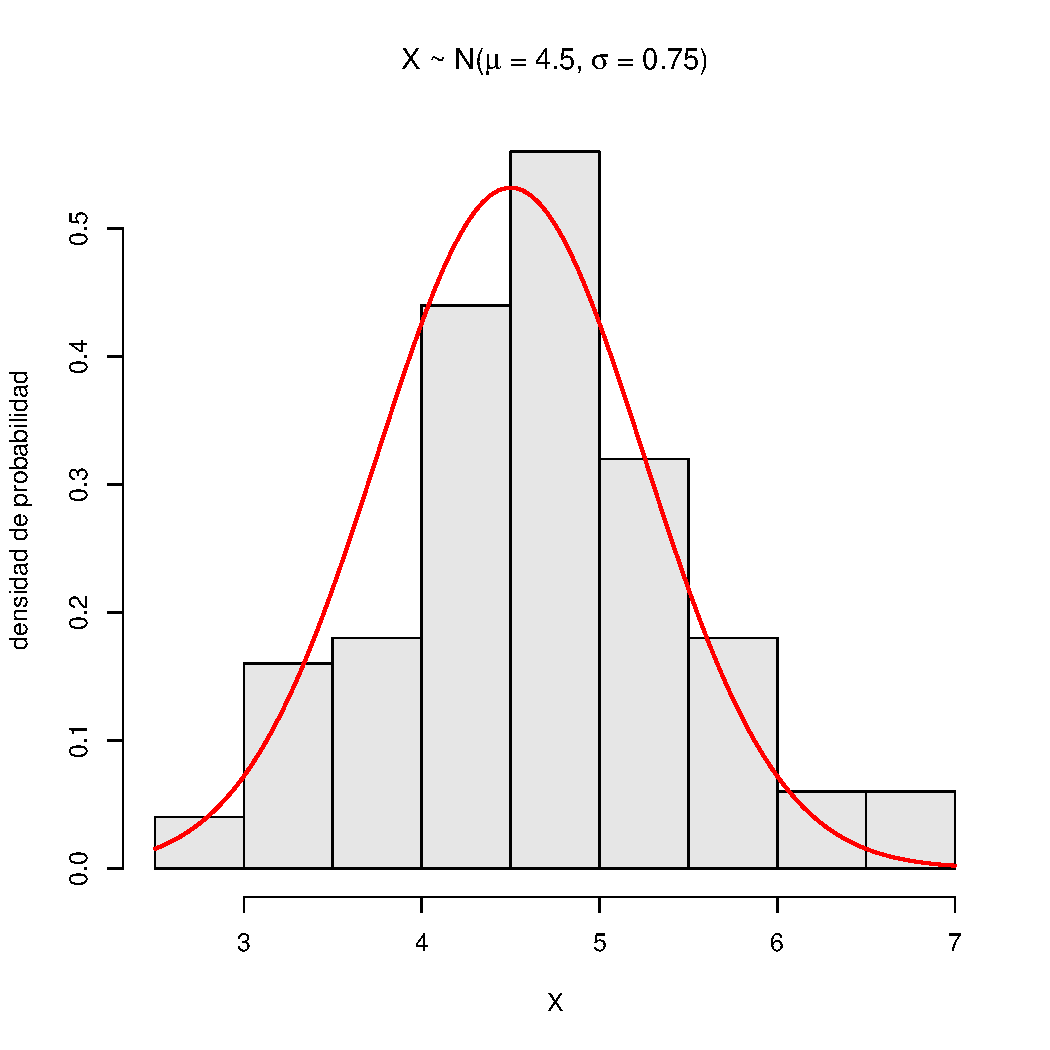
\includegraphics[width=\maxwidth]{figure/unnamed-chunk-6-1} 

\end{knitrout}


\end{document}
